\documentclass[11pt]{report}

% I want back references in my bibliography.
\usepackage[pagebackref,hidelinks]{hyperref}
% The following formats the back references nicely.
\renewcommand*{\backref}[1]{}
\renewcommand*{\backrefalt}[4]{[{%
    \ifcase #1 Not cited.%
          \or Cited on page~#2.%
          \else Cited on pages #2.%
    \fi%
    }]}
% Color for... color.
\usepackage{color}
% Need this for figures
\usepackage{graphicx}
% This may include the bibliography in the table of contents
\usepackage[numbib]{tocbibind}
% Slightly neater way of doing units.
\usepackage{units}
% Glossary package for acronyms.
\usepackage[nonumberlist]{glossaries}%[nonumberlist,nohypertypes={glossary},acronym]
\setglossarysection{subsubsection} % No page break on \printglossary
\renewcommand{\glossarysection}[2][]{} % No glossary title.

\newacronym{cdi}
    {CDI}{coherent diffractive imaging}

\newacronym{odt}
    {ODT}{optical dipole trap}

\newacronym{otr}
    {OTR}{optical transition radiation}
    
\newacronym{bec}
    {BEC}{Bose-Einstein condensate}

\newacronym{fort}
    {FORT}{far-off-resonance trap}

\newacronym{ta}
    {TA}{tapered amplifier}

\newacronym{caes}
    {CAES}{cold-atom electron source}

\newacronym{cais}
    {CAIS}{cold-atom ion source}

\newacronym{caeis}
    {CAEIS}{cold-atom electron and ion source}

\newacronym{xfel}
    {XFEL}{X-ray free electron laser}

\newacronym{mot}
    {MOT}{magneto-optical trap}

\newacronym{ecdl}
    {ECDL}{external cavity diode laser}

\newacronym{aom}
    {AOM}{acousto-optic modulator}

\newacronym{eom}
    {EOM}{electro-optic modulator}

\newacronym{slm}
    {SLM}{spatial light modulator}

\newacronym{mopa}
    {MOPA}{master-oscillator power amplifier}

\newacronym{na}
    {NA}{numerical aperture}

\newacronym{ar}
    {AR}{anti-reflection}

\newacronym{ccd}
    {CCD}{charge-coupled device}

\newacronym{cro}
    {CRO}{cathode ray oscilloscope}

\newacronym{pbs}
    {PBS}{polarising beam splitter}

\newacronym{bs}
    {BS}{beam splitter}

\newacronym{npbs}
    {NPBS}{non-polarising beam splitter}

\newacronym{tec}
    {TEC}{thermo-electric cooler}

\newacronym{cw}
    {CW}{continuous wave}

\newacronym{mcp}
    {MCP}{microchannel plate}

\newacronym{fwhm}
    {FWHM}{full-width half maximum}

\newacronym{pdh}
    {PDH}{Pound-Drever-Hall}

\newacronym{ps}
    {PS}{polarisation spectroscopy}

\newacronym{psf}
    {PSF}{point spread function}

\newacronym{obe}
    {OBE}{optical Bloch equation}
    
\newacronym{davll}
    {DAVLL}{dichroic atomic vapour laser lock}

\newacronym{mts}
    {MTS}{modulation transfer spectroscopy}

\newacronym{snr}
    {SNR}{signal-to-noise ratio}

\newacronym{lsd}
    {LSP}{linear spectral density}
    
\newacronym{psd}
    {PSD}{power spectral density}
    
\newacronym{piezo}
    {PZT}{piezoelectric transducer}

\newacronym{rms}
    {RMS}{root mean square}
    
\newacronym{sa}
    {SA}{saturated absorption spectroscopy}

\newacronym{fib}
    {FIB}{focused ion beam}

\newacronym{rf}
    {RF}{radio frequency}
    
\newacronym{ued}
    {UED}{ultrafast electron diffraction}

\newacronym{tem}
    {TEM}{transmission electron miscroscopy}

\newacronym{fsr}
    {FSR}{free-spectral range}

\newacronym{rempe}
    {REMPE}{resonace-enhanced multiphoton excitation}

\newacronym{tcmpe}
    {TCMPE}{two-colour multiphoton excitation}
\makeglossaries

\begin{document}

% Title page
\title{Thesis}

\author{Joshua Torrance}

\pagenumbering{alph} % Title page becomes a so backrefs to 1 go to the right place.
\maketitle

\pagenumbering{roman}

% Front matter
\chapter*{Abstract}
\addcontentsline{toc}{chapter}{Abstract}

The understanding of atomic structures and processes is continually improving with the great technological development in imaging techniques.
Ultrafast electron and X-ray techniques are able to perform measurements at atomic lengths and timescales and both these techniques require the generation of high-brightness ultrashort-duration electron bunches.
Electron techniques directly use these short bright bunches and in \glspl{xfel} the electron bunches are used to generate short bright bunches of X-ray.

It is hoped that \glspl{caeis} will also be able to produce ultrashort high-brightness electron bunches that are brighter than current sources due to the unique method of generating electrons used by these sources.
\Glspl{caeis} generate electrons via near-threshold ionisation from an ultracold atomic gas and has been shown to create electrons bunches with temperature as low as \unit[10]{K}.
Conventional photocathode sources have temperatures of thousands of Kelvin and thus \glspl{caeis} have the potential to produce brighter electron bunches.
\Gls{caeis} are also capable of producing extremely cold ion bunches and show great promise as an ion source for ion milling and microscopy.

This thesis describes a number of developments involved with the \gls{caeis} project at the University of Melbourne, in particular pushing the boundaries of laser frequency stabilisation, and a new technique for measuring the brightness of charged particle bunches.
A number of smaller developments and investigations are presented along with the newest diffraction measurements.

Laser frequency stabilisation is an essential component of the \gls{caeis} and many other applications including metrology, spectroscopy and laser cooling.
The high-bandwidth of the laser stabilisation technique polarisation spectroscopy has not previously been fully utilised and by using high-bandwidth feedback laser linewidth can be narrowed to much less than \unit[1]{kHz}, two orders of magnitude better than previously reported.

Brightness is the most comprehensive figure of merit for charged particle beams and a new technique for measuring the brightness with time-resolution is presented.
The technique achieves time-resolved brightness measurements by streaking one-dimensional pepperpot measurements across the detector.
Time-resolved brightness measurements have the potential to reveal information related to the ionisation processes used in \glspl{caeis} and can show the efficacy of techniques used to counter the effects of space charge in the beams produced from a \gls{caeis}.

The performance of the \gls{caeis} apparatus operating in its normal pulsed mode is compared to continuous operation with a focus on the beam current and electron trajectory stability.
The beam quality was also improved by identifying an astigmatism in the beam and correcting it with a 3D printed quadrupole lens.
Virtually all the beam measurements presented here utilise the image processing techniques that allow for multi-shot averaging despite the inconvenient instabilities in the electron beam trajectories.

This iteration of a \glspl{caeis} was able to produce ultrashort-duration electron bunches and these have been used to demonstrate ultrafast electron diffraction from thin gold foils.
This is an important step along the path to being able to perform ultrafast single-shot \gls{cdi} and next iteration of the \gls{caeis} should have sufficient current to demonstrate \emph{single-shot} ultrafast diffraction and then move on to \gls{cdi}.
\chapter*{Acknowledgements}
\addcontentsline{toc}{chapter}{Acknowledgements}

Acknowledgements go here.

\chapter*{Contributions}
\addcontentsline{toc}{chapter}{Contributions}

This thesis presents work I was involved with as a member of the Atom Optics group in the School of Physics at the Unisversity of Melbourne.
All work in this thesis was conducted by me, unless mentioned below:
\begin{itemize}
\item The Cold-Atom Electron and Ion Source: The experimental apparatus was designed, contructed, and improved by other members of the group before my research with it began.
Some of the members of the group that have worked on the apparatus are
Andrew McCulloch, Dene Murphy, Corey Putkunz, Robert Scholten, David Sheludko, Sebastian Saliba, Ben Sparkes, Rory Speirs, Richard Taylor, and Daniel Thompson.
\item The high-bandwidth polarisation spectroscopy work described in Chapter~\ref{chapter:polspec} was conducted with much help and advice from Robert Scholten, Ben Sparkes as well as Lincoln Turner from Monash University. Alex Slavec from MOGLabs was also instrumental in this work as he engineered the high-bandwidth modifications for the MOGLabs lasers used.
\item The results described in Chapter~\ref{chapter:diffraction} built on work done by Rory Speirs, published in Reference~\cite{speirs_single-shot_2015}, and conducted with much advice from Rory.
\item The deflectors used to streak the electron beam in Chapter~\ref{chapter:emittance} were supplied a voltage with electronics designed and built by Rory Speirs and the deflector plates were designed by Andrew McCulloch.
\end{itemize}

\tableofcontents

 \chapter{Introduction}
 
\pagenumbering{arabic}
\setcounter{page}{1}

Molecular imaging has provided science with great advances during it's history, such as X-ray crystallography determining the helical structure of DNA in 1953~\cite{watson_molecular_1953} and structure of myoglobin and haemoglobin in 1962~\cite{kendrew_x-ray_1957}.
The \gls{caeis} at the University of Melbourne is an ongoing project that aims to develop a source capable of achieving the `holy grail' of scientific imaging, the `molecular movie'~\cite{dwyer_femtosecond_2006,sciaini_femtosecond_2011}.
A \gls{caeis} also has potential applications with \gls{fib} techniques~\cite{mcclelland_bright_2016}, and as particle source for accelerators such as synchrotrons and \glspl{xfel} for \gls{cdi} of non-crystalline targets~\cite{van_oudheusden_electron_2007, zhu_future_2015, mcculloch_cold_2016}.



{\color{red}
Some kind of introduction for everything will go here.

Motivate CAES. Imaging of things is important. Membrane proteins, cystallisation. What else can we image with it? What else can we study with it? Ion source.

Briefly motivate part 1 and part 2.}

\section{Making the `Molecular Movie'}

Being able to observe molecular dynamics at an atomic spatial and temporal scale could provide great insight into some of the basic processes of biology and chemistry.
The fabled `molecular movie' refers to capturing the atomic motions of molecular systems as they undergo some transition such as a chemical reaction, protein folding or melting.
Molecular movies could provide greater understanding of important biological reactions such as photosynthesis or oxygen transport by haemoglobin.

One of the stepping stones towards molecular movies is single-shot imaging of non-crystalline molecules which would allow structural determination of membrane proteins, an essential step in rational drug design~\cite{hardy_atomic_1987, barrett_discovering_1999, pinto_influenza_1992}.
One of the main techniques in stuctural determination of crystalline targets is electron diffraction which, along with X-ray and neutron methods~\cite{cullity_elements_2001,bacon_x-ray_2013}, has be utilised in structural determination of many materials with atomic resolution.
Continuing research into real-space and diffraction imaging techniques is aiding in the understanding of a growing range of samples as well as providing new types of information on the sample under investigation.

Ultrafast imaging techniques are a relatively recent development and they provide the opportunity to study electronic and atomic dynamics.
Ultrafast techniques also provide an avenue for the imaging of structures that, to date, cannot be imaged by cyrstallographic techniques as some of these techniques should be applicable to uncrystallised samples with imaging being faster than damage processes~\cite{gaffney_imaging_2007,barty_ultrafast_2008,miao_beyond_2015}.
In the past the greatest success with structural determination has been acheived with crystallography which is limited by to samples that can be crystallised.
There are a large number of biological proteins of interest, particularly membrane proteins, that cannot be crystallised and developements in ultrafast imaging techniques is providing a route towards structural determination without crystallisation~\cite{dauter_current_2006,levitt_nature_2009}, cryogenic electron microscopy is also making headway in this area~\cite{henderson_model_1990,zhou_towards_2008}.
Both X-ray and electron imaging techniques are limited by the capabilities of their sources which are undergoing continual developement, in the realms of fundamental physics and engineering.
The techniques using X-rays and electrons each have different advantages and disadvantages with regards to dynamic imaging and structural determination and they often give complementary information.

Some recent results from X-ray sources are well on the way to producing molecular movies~\cite{pande_femtosecond_2016,nango_three-dimensional_2016}.

\subsection{Imaging Targets}

Membrane proteins.
Chemical reactions.


\subsection{Requirements}

Ultra-fast, single-shot, orientation, flux, coherence.

\subsection{X-rays}

XFELs

\subsection{Electrons}

\subsection{Pump-Probe}

\section{Cold-atom electron sources}

\subsection{Developments}

Arbitrary shaping, charged partical dynamics, diffraction.
\subsection{Ion Source}

\section{Thesis Outline}

\subsection{Part I}

\subsection{Part II}

% The following two lines need to be in the first chapter to get Arabic page numbers.
%\pagenumbering{arabic}
%\setcounter{page}{1}
\part[Polarisation Spectroscopy]{Polarisation Spectroscopy\\
\vspace{1cm}
\LARGE Pushing the Limits of Polarisation Spectroscopy as a Laser Frequency Reference}
\chapter{Introduction}

Laser frequency stabilisation is an essential tool for atomic physics experiments, without it experiments involving \glspl{bec}, atomic clocks and many more would not be possible~\cite{anderson_observation_1995,ye_quantum_2008}.
There are a plethora of techniques available for laser frequency stabilisation each with numerous advantages and disadvantages.

\Gls{ps} is one such technique that will be discussed in detail~\cite{demtroder_laser_2003}.
\Gls{ps} was first described by Wieman and H\"anch in 1976 as, ``...a sensitive new method of Doppler-free spectroscopy, monitoring the nonlinear interaction of two monochromatic laser beams in an absorbing gas via changes in light polarisation."~\cite{wieman_doppler-free_1976}
This chapter provides an overview of laser frequency stabilisation, a detailed discussion of the physics of \gls{ps} followed by details on the implementation and measurement of high bandwidth frequency stabilisation using \gls{ps}.

\section{Laser Frequency Stabilisation}

Laser frequency stabilisation describes a number of techniques that are used to reduce the temporal frequency spread of a laser's frequency.
This can range from weak frequency stabilisation keeping the centre frequency of a laser at a particular point to convoluted frequency narrowing techniques that attempt to reduce laser linewidth to sub-hertz levels.
Typically these techniques use some reference to measure frequency deviation from a given frequency and provide negative feedback to the laser, using a servo system, to keep it at the target frequency.

The efficacy of stabilisation techniques can be described by width of the frequency distribution of the laser, called the linewidth.
Width is usually refers to either the \gls{fwhm} or \gls{rms} width about the central frequency.
Linewidth can describe short or long timescale measurements.
Short measurements, usually less than a second measurement, are used to describe the linewidth of laser whereas long timescale measurement, hours or days in duration, are used to describe the drift of the laser central frequency over time.

There are a number of traits that are desirable in a laser frequency stabilization scheme including the ability to stabilize to an absolute atomic reference, absence of frequency or amplitude modulation, high bandwidth to achieve low spectral linewidth, large capture range, low complexity and low cost.

There are a large number of available techniques and variations on techniques for stabilization each with different advantages and drawbacks.
These techniques include
\begin{itemize}
\item \gls{sa}~\cite{haroche_theory_1972, maguire_theoretical_2006, cuneo_optically_1994, preston_doppler-free_1996, saliba_linewidths_2009},
\item \gls{davll}~\cite{corwin_frequency-stabilized_1998, millett-sikking_davll_2007},
\item \gls{mts}~\cite{shirley_modulation_1982, mccarron_modulation_2008, xiang-hui_ultra-stable_2009},
\item Sagnac interferometry~\cite{robins_Interferometric_2002, jundt_non-linear_2003},
\item \acrfull{ps}~\cite{wieman_doppler-free_1976, lancaster_polarisation_1999, yoshikawa_frequency_2003, harris_polarization_2006, pearman_polarization_2002, tiwari_laser_2006, do_polarization_2008, torii_laser-phase_2012}
\item \gls{pdh}~\cite{drever_laser_1983} and
\item H\"ansch Couillaud stabilisation~\cite{hansch_laser_1980}.
\end{itemize}
Some of these techniques will be discussed later on in this chapter.

\section{Feedback Methods}

Stabilisation techniques require some kind of feedback to the laser in order to keep it at the desired frequency.
There are a few common ways of providing feedback to lasers, the focus here will be on diode lasers, particularly \glspl{ecdl}.

\subsection{Current Feedback}

Diode lasers require an electric current in order to function and this current can be used to control the output frequency of the laser.
The front and rear facets of laser diodes are reflecting forming an optical cavity.
The optical cavity support standing waves of particular wavelengths which serve to enhance the stimulated emission essential to lasing.
The electrical current passing through a laser diode will cause an increase in temperature of the diode which in turn increases the size of the cavity and the supported standing wave wavelength.
Increasing the temperature also affects the band gaps in the crystal such that an increase in temperature causes an increase in wavelength.
Thus altering the current supply to the laser can be use to control the central output frequency of the laser.

{\color{red} Verify these and provide citations.}

To talk about:
\begin{itemize}
\item Typical feedback bandwidths.
\item Grating feedback.
\item Fast feedback - complications (isolation from ground, phase lag...).
\end{itemize}


\section{Noise}
Thermal noise can affect the alignment of optics, the efficiency and polarisation of light transmitted through fibres, atomic vapour cell opacity and the intensity and frequency of light emitted from laser diodes, not to mention mode hops.

Noise in the electronic environment can also cause frequency instability. Noise on the power supply to the laser diode affects the intensity and frequency of the light emitted.

In certain applications {\color{red}(such as?? imaging?)} intensity noise can be as much as a drawback as frequency noise and with some frequency discrimination methods intensity noise is interpreted as frequency noise which the servo would then attempt to correct for thus inducing frequency noise.

Feedback to laser systems typically takes the form of modulation of either the current supply to the diode or the voltage to a piezo that controls the angle of the grating in an \gls{ecdl}.
Temperature feedback has also been used to maintain frequency stability {\color{red}[find that paper again]}.
The bandwidth of current feedback tends to range from \unit[0]{Hz} to MHz~\cite{ludlow_compact_2007}{\color{red}[cite my paper here?]}.
Piezo response is significantly slower ranging from \unit[0]{Hz} to \unit[100]{kHz}.

{\color{red}Frequency ranges of noise.}
{\color{red}More detail? More References on noise in general.}

Bleh.
\Glspl{ecdl} subjected to mechanical vibrations will experience frequency noise as the alignment of the light coupled back into the diode off the grating varies.
Vibrations can also affect the alignment, and thus transmitted power, of laser through optical fibres, optical isolators and through apertures.

\section{Stabilisation Techniques}
\subsection{Saturated Absorption Spectroscopy}
\Gls{sa} is a simple and common technique for laser frequency stabilisation~\cite{demtroder_laser_2003}.
 
\begin{figure}
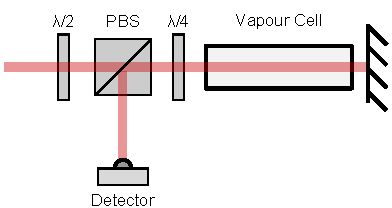
\includegraphics[width=\linewidth]{part1/Figs/SatAbs.pdf}
\caption{Saturated absorption spectroscopy.}
\label{figure:satabs}
\end{figure}

\subsection{Polarisation Spectroscopy}

Summary of PS.

Pol Spec developments

It has been shown previously that \gls*{ps} can be used to reduce the linewidth of a distributed feedback diode from \unit[2]{MHz} to \unit[20]{kHz}~\cite{torii_laser-phase_2012} and of \glspl*{ecdl} to \unit[65]{kHz}
~\cite{yoshikawa_frequency_2003}.

Balanced polarimeter.\cite{pearman_polarization_2002,yoshikawa_frequency_2003}

Bi-polarisation spectroscopy.\cite{tiwari_laser_2006}


\subsection{Pound Drever Hall}

The \gls{pdh} technique is the standard for laser frequency linewidth reduction.\cite{drever_laser_1983}
\gls{pdh} uses an optical cavity as a frequency reference and an \gls{eom} to modulate the the light incident to the cavity.

More detail. Some maths. What linewidth can it achieve?\cite{ludlow_compact_2007}

\begin{figure}
\centering
\includegraphics[width=\linewidth]{part1/Figs/pdh.jpg}
\caption{A beautiful \gls{pdh} schematic.}
\end{figure}
\subsubsection{Dichroic Atomic Vapour Laser Lock}
\Gls{davll} works by....

It can achieve linewidths of....

\subsection{Modulation Transfer Spectroscopy}
\Gls{mts}...

It can achieve linewidths of...\cite{negnevitsky_wideband_2013}

\subsection{Other Techniques}

Any others?




\part{Coherent Diffractive Imaging with a Cold-Atom Electron Source}

\appendix
\chapter{Glossary}
\printglossary

% References
\bibliographystyle{unsrt}
\renewcommand\bibname{References}
\bibliography{Library}

\end{document}
